\section{考察}
前章では干渉パターンを4つの要素に分解し、位相に関係した2つのパラメータ$B,C$については実験結果を理論がよく説明することを見た。しかし波の水深に関係した2つのパラメータ$A,D$については実験結果と理論との間に相違が見られた。この章ではこの相違を説明するために2つの異なる仮説を立て、それぞれ仮説の下で実験結果がうまく説明できるかを考察する。

\subsection{バックグラウンド}
干渉を見る波長領域の中にミラーで反射されていない中性子が混ざっていたとすると、その分干渉波の振動中心は粒子数の多い方にずれ、観測確率として見たときの干渉波の振幅は小さくなることが予想される。

\paragraph{形}
バックグラウンドの分布としてどのような形を仮定するべきか検討を行う。次の図\ref{Discussion2_fig_flipperoff}はスピンフリッパーをOFFにしたときの規格化粒子数の波長分布である。0\AA 付近に高速中性子の立ち上がりが、3.2\AA 付近に反射中性子のピークが見える。そしてその間1\AA 付近にもピークが確認できる。図\ref{Discussion_fig_mirroroff}はミラーを置かずに測定を行ったときの検出粒子数の波長分布であり、1\AA 付近のピークはKUANSからの熱中性子のピークである。すなわち図\ref{Discussion2_fig_flipperoff}の1\AA 付近のピークはミラーで反射されずに検出された熱中性子の一部であると考えられる。
\begin{figure}[H]
%\begin{minipage}{0.5\hsize}
\centering
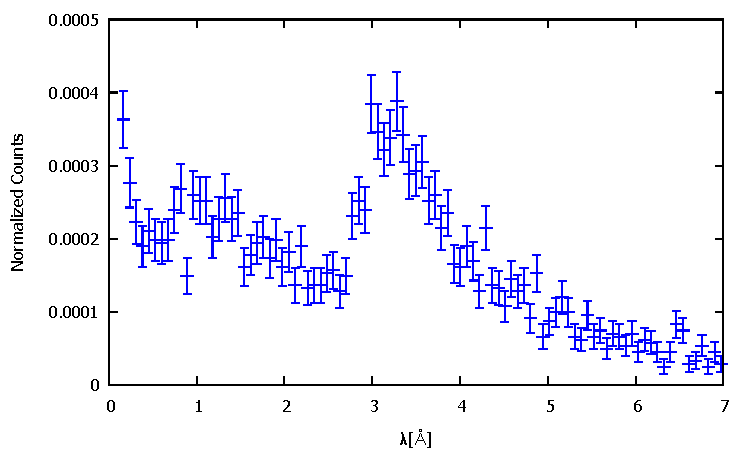
\includegraphics[width=9cm]{discussion/BG/flipperoff.pdf}
\caption{フリッパーOFF時の規格化粒子数波長分布(\ce{^3He}比例計数管による測定)}\label{Discussion2_fig_flipperoff}
%\end{minipage}
%\begin{minipage}{0.5\hsize}
%\centering
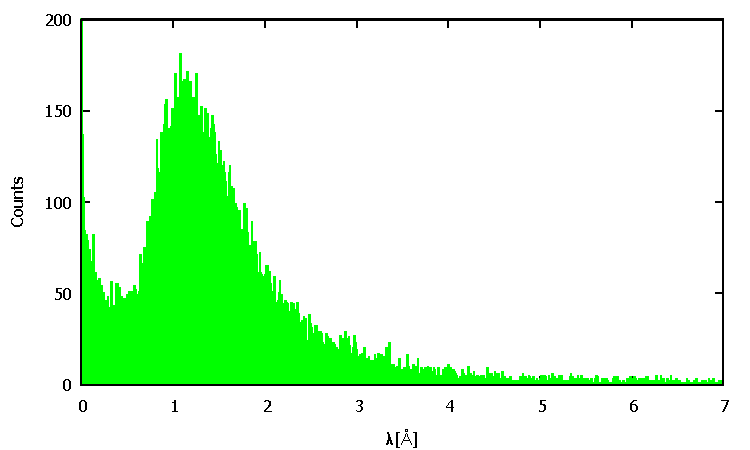
\includegraphics[width=9cm]{discussion/BG/mirroroff.pdf}
\caption{ミラーを置かずに測定した粒子数波長分布(RPMT検出器による測定)}\label{Discussion2_fig_flipperoff}
%\end{minipage}
\end{figure}

次の図\ref{Discussion2_fig_detectormove}はスピンフリッパーOFF時に検出器の$y$座標を、図\ref{Discussion2_fig_flipperoff}の測定位置を$y=0$として、$y=-18,-9,0,+9,+18$mmと動かしたときの規格化粒子数波長分布である。図\ref{Discussion2_fig_detectormove}から$y=0$に近づくにつれ反射中性子のピークが大きくなっていくことがわかるが、5.5\AA 以上の長波長における分布は検出器の位置を動かしてもほとんど一定である。すなわち5.5\AA 以上の長波長においても消えない一定数のバックグラウンドが存在する。
\begin{figure}[h]
\begin{minipage}{0.5\hsize}
\centering
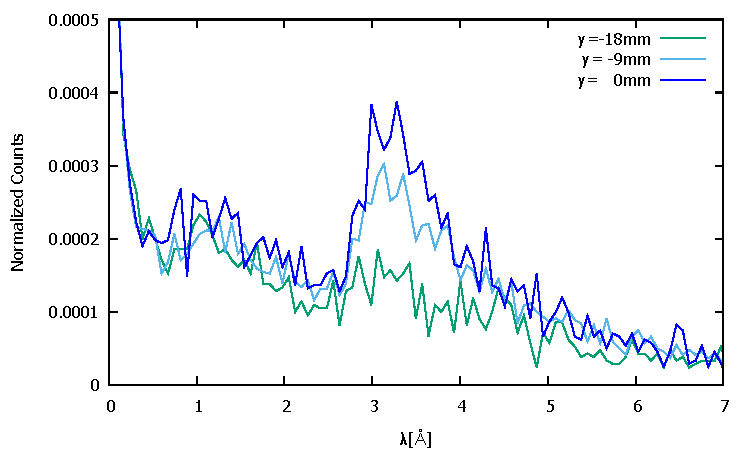
\includegraphics[width=\hsize]{discussion/BG/flippermove1.pdf}
\end{minipage}
\begin{minipage}{0.5\hsize}
\centering
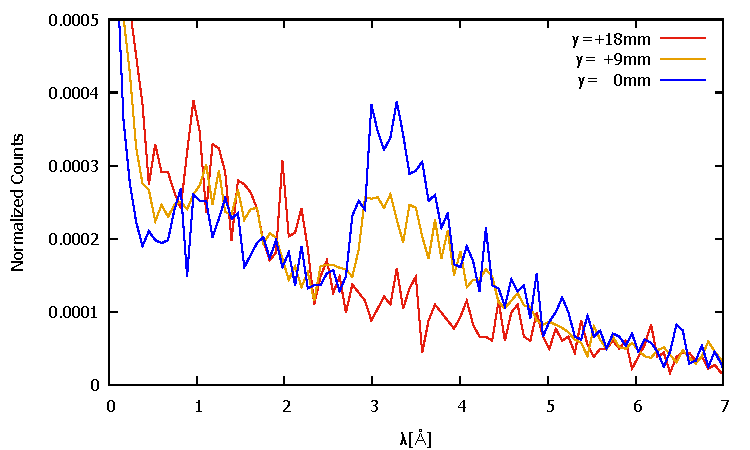
\includegraphics[width=\hsize]{discussion/BG/flippermove2.pdf}
\end{minipage}
\caption{検出器の位置を動かしたときの規格化粒子数}\label{Discussion2_fig_detectormove}
\end{figure}

以上からバックグラウンドとしてあるピークを持ち長波長で消えないものを取りたい。そこで最もシンプルにガウシアンに定数項のついた$a\exp(-(x-b)^2/2c^2)+d$の形を採用する。なおもともとの熱中性子はMaxwell分布に従うが、バックグラウンドとして検出されたものは壁などで反射された成分などを含み元の分布とは異なると考えられるため、シンプルな形を採用した。図\ref{Discussion2_fig_flipperoff}を反射成分を除く0.5-2.5と5.5-7\AA の範囲でフィッティングした結果を図\ref{Discussion2_fig_backfit}に表し、各パラメータの値を表\ref{Discussion2_tbl_backfit}に示す。

\begin{figure}[H]
\begin{minipage}{0.7\hsize}
\centering
%\vspace{2.5cm}
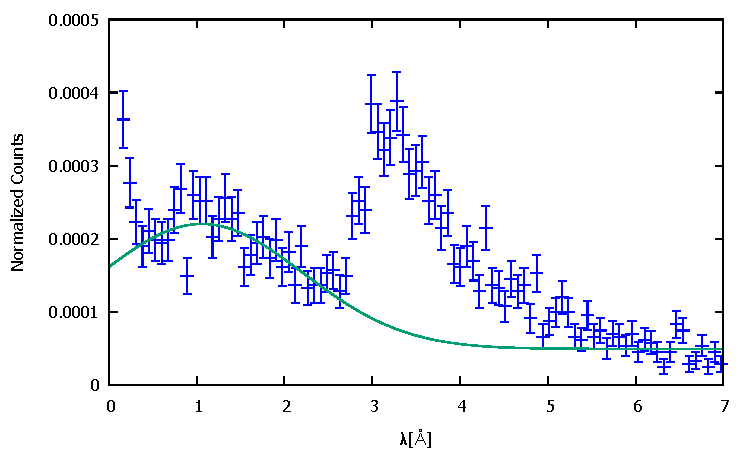
\includegraphics[width=10cm]{discussion/BG/background.pdf}
\caption{バックグラウンド} \label{Discussion2_fig_backfit}
\end{minipage}
\begin{minipage}{0.3\hsize}
\centering
\makeatletter
\def\@captype{table}
\makeatother
\caption{各パラメータ} \label{Discussion2_tbl_backfit}
\begin{tabular}{|c|c|} \hline
$a$&$1.7\times 10^{-4}\pm 1\times10^{-5}$\\ \hline
$b$&$1.1\pm0.2$\\ \hline
$c$&$1.1\pm0.2$\\ \hline
$d$&$4.9\times 10^{-5}\pm4\times 10^{-6}$\\ \hline
\end{tabular}
\end{minipage}
\end{figure}

\paragraph{結果}
章と同様に次の手順でバックグラウンドを考慮した場合のスピン上向き中性子観測確率の干渉パターンとフィッティングパラメータ$A,B,C,D$を得た。
\begin{enumerate}
\item シフタコイル電流を変えていったときの規格化粒子数の波長分布(図\ref{Discussion2_fig_NC})からバックグラウンドを取り除いた分布(図\ref{Discussion2_fig_NC_b})を得た
\item 図\ref{Discussion2_fig_NC_b}の分布において種々の中心波長$\pm0.07$\AA の波長領域に含まれる規格化粒子数を数え、シフタコイル電流を横軸とした干渉パターン(図\ref{Discussion2_fig_IF_nb})を得た
\item 干渉パターンを$-A'\cos(Bx+C)+D'$でフィットした
\item フリッパーOFF時の規格化粒子数からバックグラウンドを除いた分布から、そろぞれの波長領域における干渉パターンの縦軸(規格化粒子数)をスピン上向き中性子の観測確率とするためのファクターを求めた
\item 図\ref{Discussion2_fig_IF_nb}を上で求めたファクターで割り、スピン上向き中性子の観測確率の干渉パターン(図\ref{Discussion2_fig_IF_rb})を得た
\item フィッティングパラメータ$A',D'$をファクターで割り、理論と比較可能なパラメータ$A,B,C,D$を得た(表\ref{Discussion2_tbl_IF_rb})
\end{enumerate}

\begin{figure}[h]
\begin{minipage}{0.33\hsize}
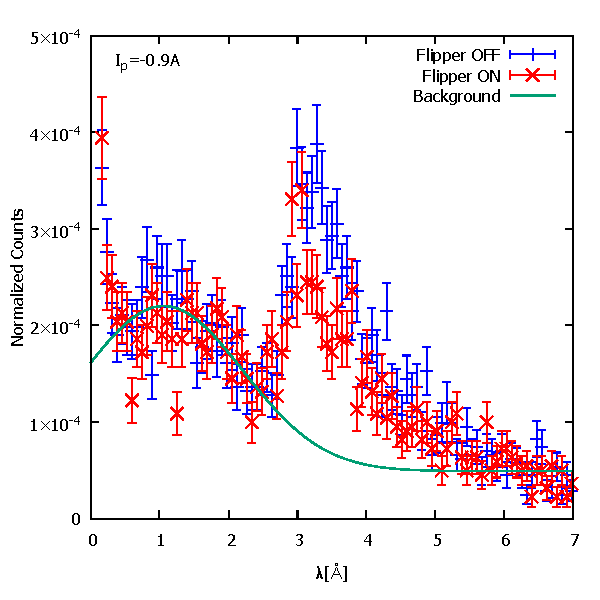
\includegraphics[width=5cm]{discussion/NC/NormalizedCounts_-9A.pdf}
\end{minipage}
\begin{minipage}{0.33\hsize}
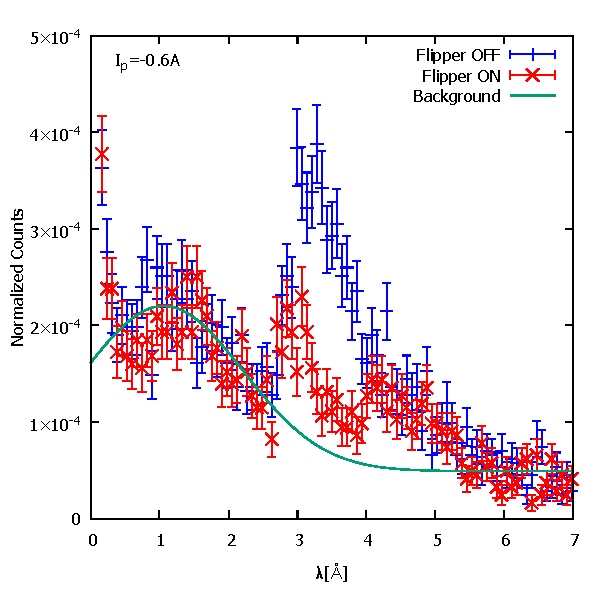
\includegraphics[width=5cm]{discussion/NC/NormalizedCounts_-6A.pdf}
\end{minipage}
\begin{minipage}{0.33\hsize}
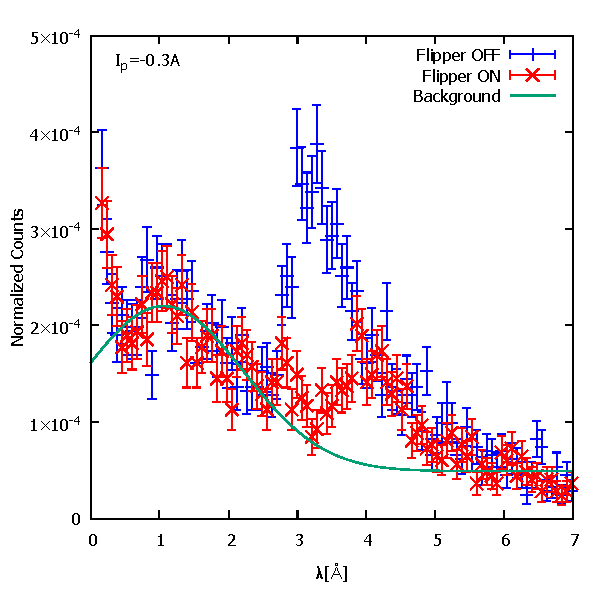
\includegraphics[width=5cm]{discussion/NC/NormalizedCounts_-3A.pdf}
\end{minipage}\\
\begin{minipage}{0.33\hsize}
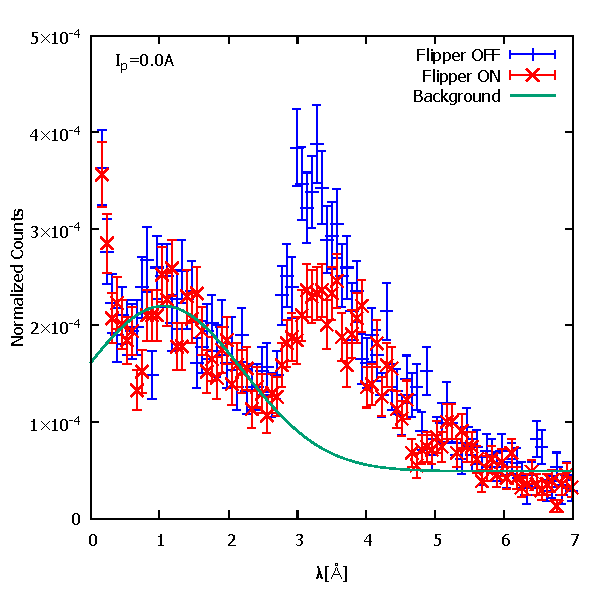
\includegraphics[width=5cm]{discussion/NC/NormalizedCounts_0A.pdf}
\end{minipage}
\begin{minipage}{0.33\hsize}
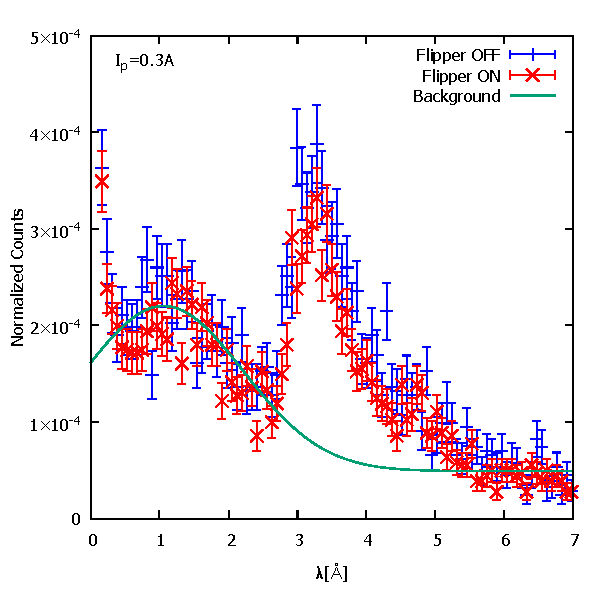
\includegraphics[width=5cm]{discussion/NC/NormalizedCounts_3A.pdf}
\end{minipage}
\begin{minipage}{0.33\hsize}
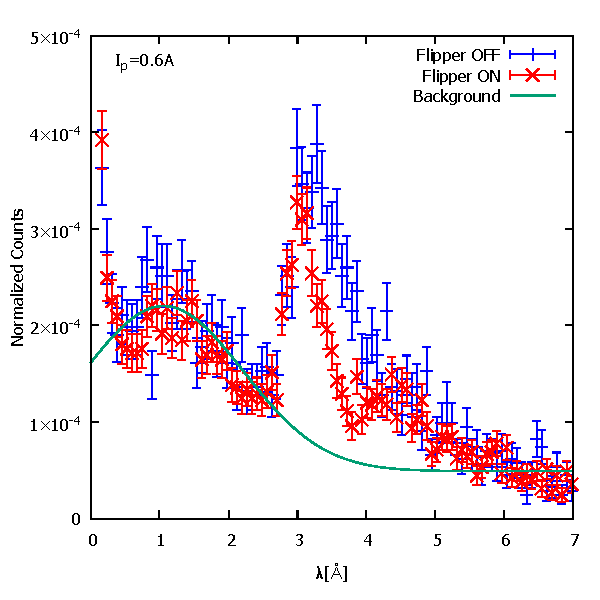
\includegraphics[width=5cm]{discussion/NC/NormalizedCounts_6A.pdf}
\end{minipage}\\
\begin{minipage}{0.33\hsize}
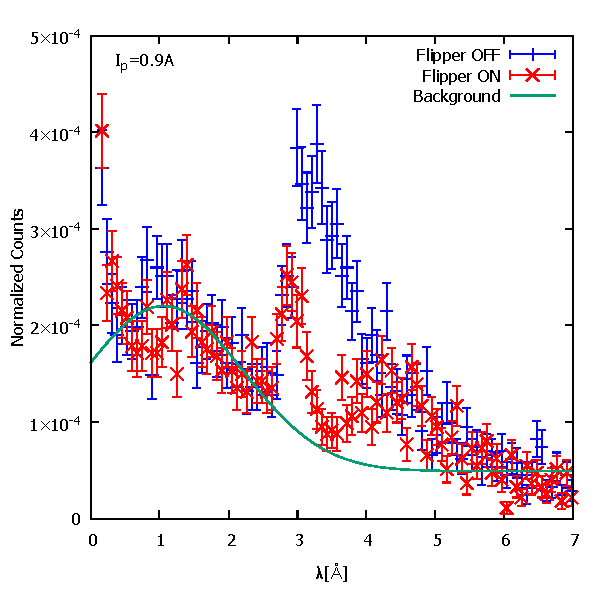
\includegraphics[width=5cm]{discussion/NC/NormalizedCounts_9A.pdf}
\end{minipage}
\begin{minipage}{0.33\hsize}
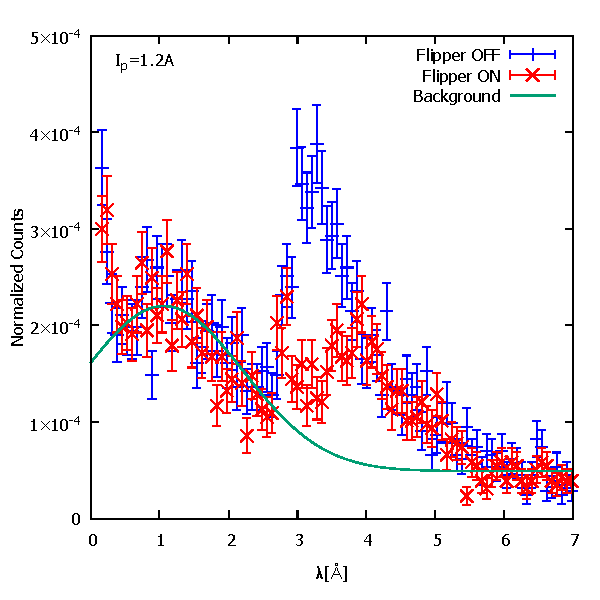
\includegraphics[width=5cm]{discussion/NC/NormalizedCounts_12A.pdf}
\end{minipage}
\begin{minipage}{0.33\hsize}
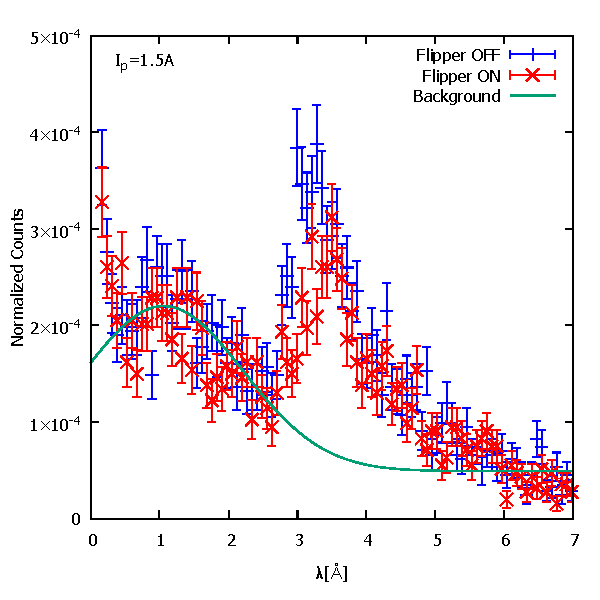
\includegraphics[width=5cm]{discussion/NC/NormalizedCounts_15A.pdf}
\end{minipage}\\
\begin{minipage}{0.33\hsize}
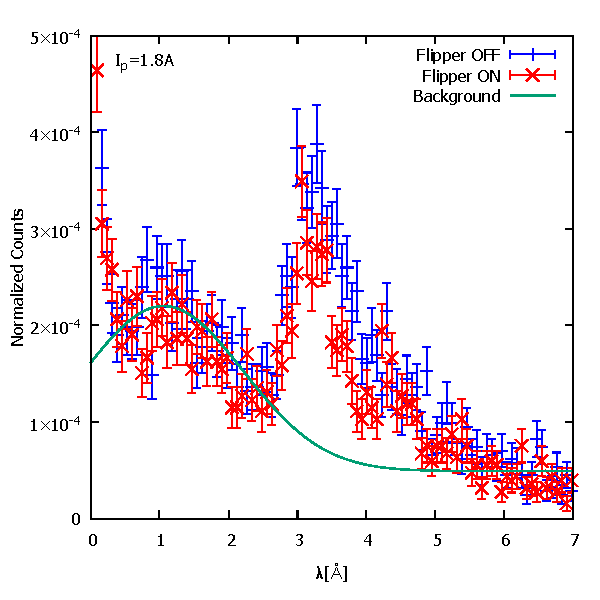
\includegraphics[width=5cm]{discussion/NC/NormalizedCounts_18A.pdf}
\end{minipage}
\begin{minipage}{0.33\hsize}
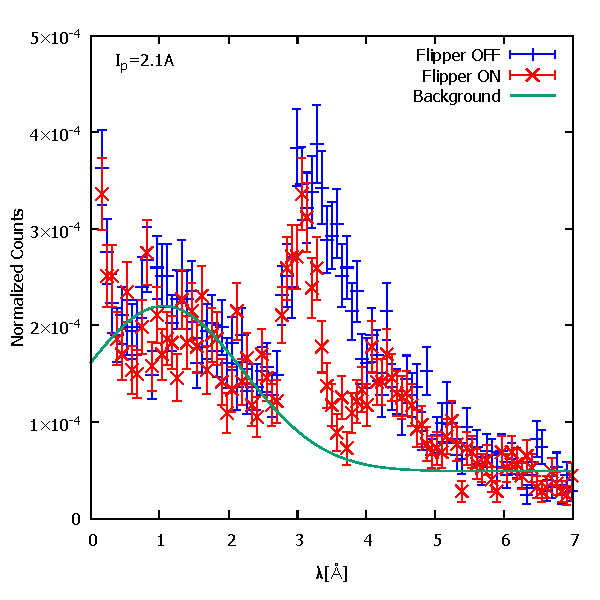
\includegraphics[width=5cm]{discussion/NC/NormalizedCounts_21A.pdf}
\end{minipage}
\begin{minipage}{0.33\hsize}
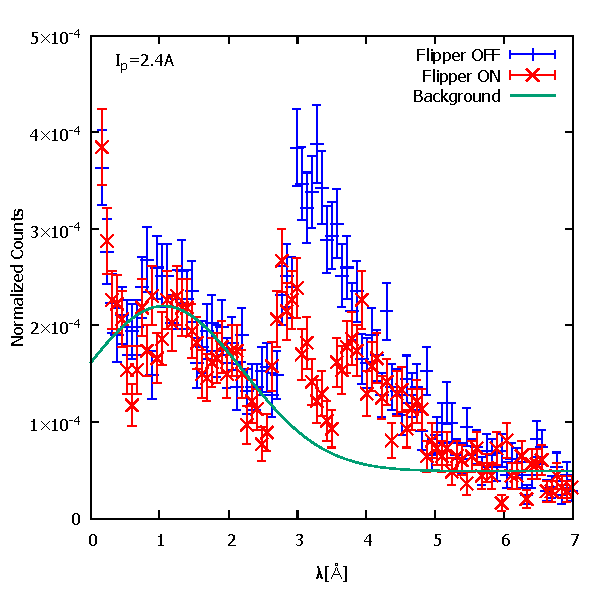
\includegraphics[width=5cm]{discussion/NC/NormalizedCounts_24A.pdf}
\end{minipage}
\caption{規格化粒子数の波長分布(バックグラウンドを引く前)}\label{Discussion2_fig_NC}
\end{figure}

\begin{figure}[h]
\begin{minipage}{0.33\hsize}
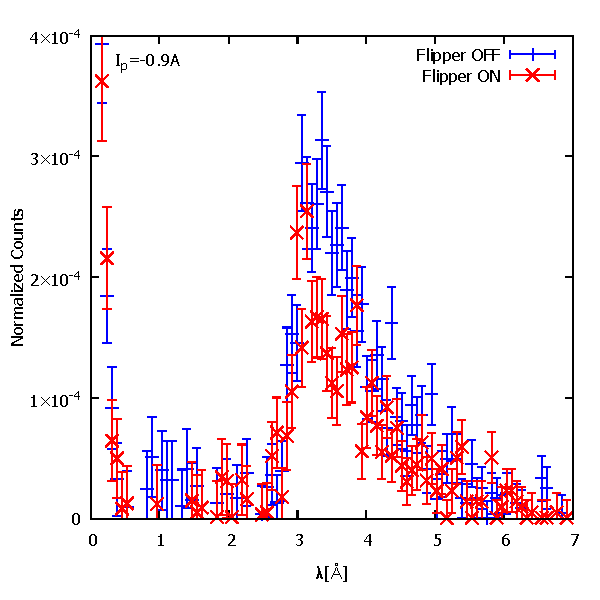
\includegraphics[width=5cm]{discussion/NC-BG/NormalizedCounts_b_-9A.pdf}
\end{minipage}
\begin{minipage}{0.33\hsize}
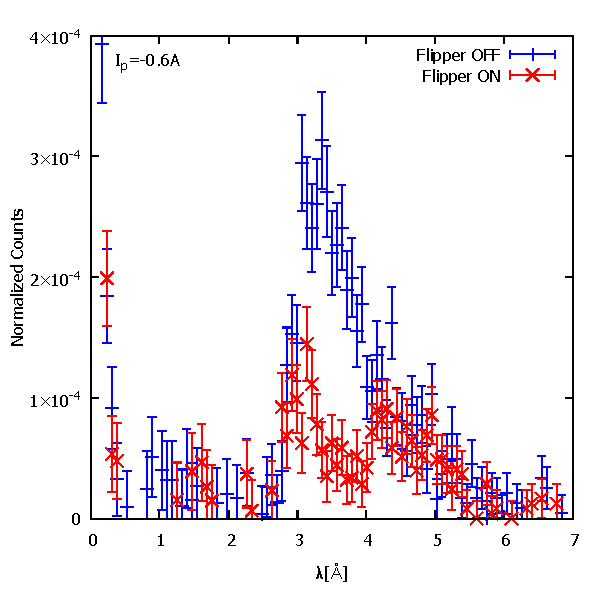
\includegraphics[width=5cm]{discussion/NC-BG/NormalizedCounts_b_-6A.pdf}
\end{minipage}
\begin{minipage}{0.33\hsize}
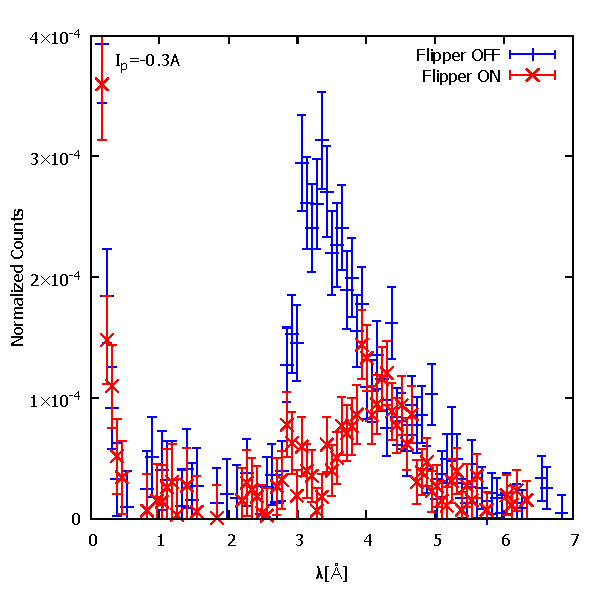
\includegraphics[width=5cm]{discussion/NC-BG/NormalizedCounts_b_-3A.pdf}
\end{minipage}\\
\begin{minipage}{0.33\hsize}
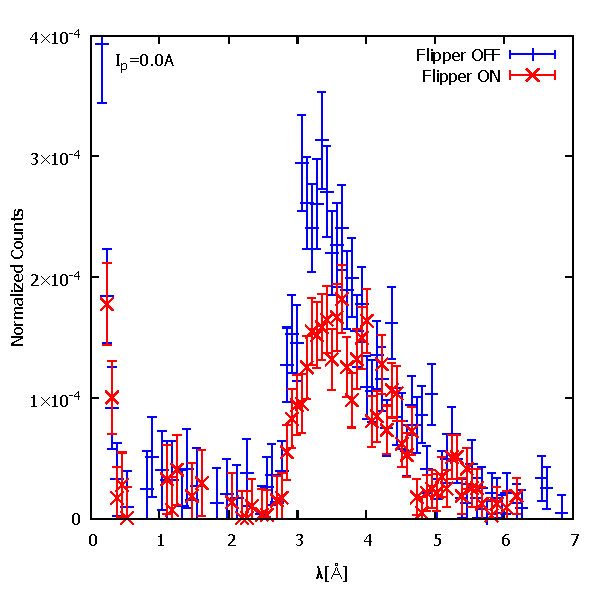
\includegraphics[width=5cm]{discussion/NC-BG/NormalizedCounts_b_0A.pdf}
\end{minipage}
\begin{minipage}{0.33\hsize}
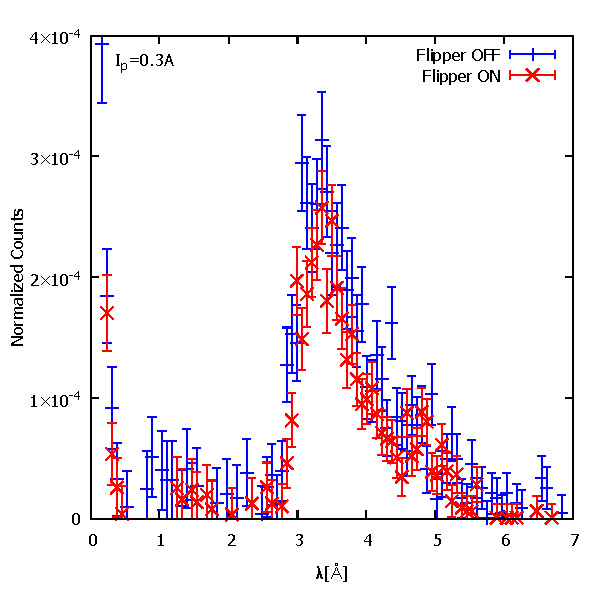
\includegraphics[width=5cm]{discussion/NC-BG/NormalizedCounts_b_3A.pdf}
\end{minipage}
\begin{minipage}{0.33\hsize}
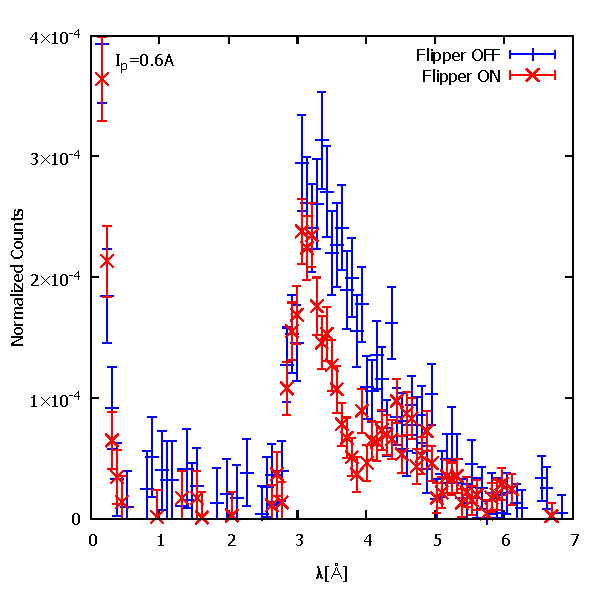
\includegraphics[width=5cm]{discussion/NC-BG/NormalizedCounts_b_6A.pdf}
\end{minipage}\\
\begin{minipage}{0.33\hsize}
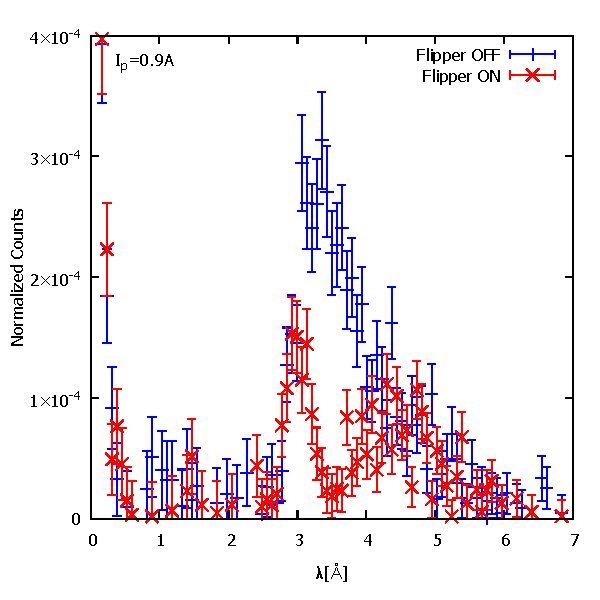
\includegraphics[width=5cm]{discussion/NC-BG/NormalizedCounts_b_9A.pdf}
\end{minipage}
\begin{minipage}{0.33\hsize}
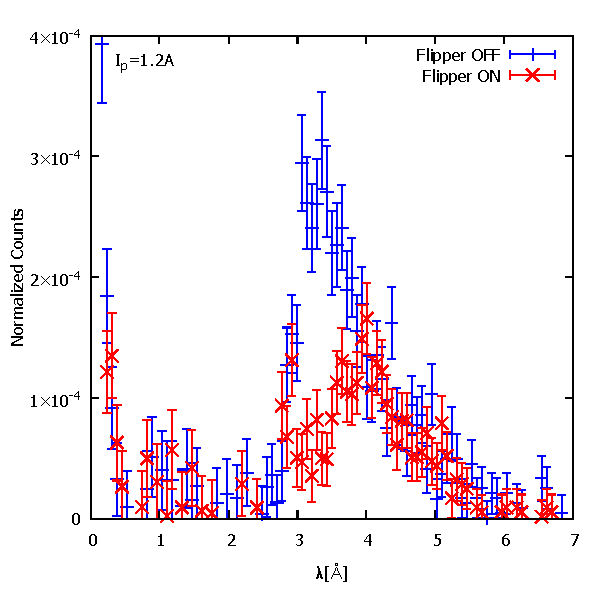
\includegraphics[width=5cm]{discussion/NC-BG/NormalizedCounts_b_12A.pdf}
\end{minipage}
\begin{minipage}{0.33\hsize}
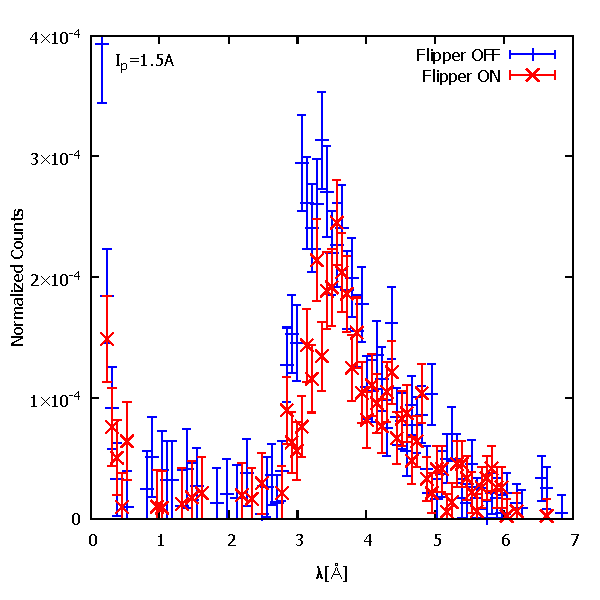
\includegraphics[width=5cm]{discussion/NC-BG/NormalizedCounts_b_15A.pdf}
\end{minipage}\\
\begin{minipage}{0.33\hsize}
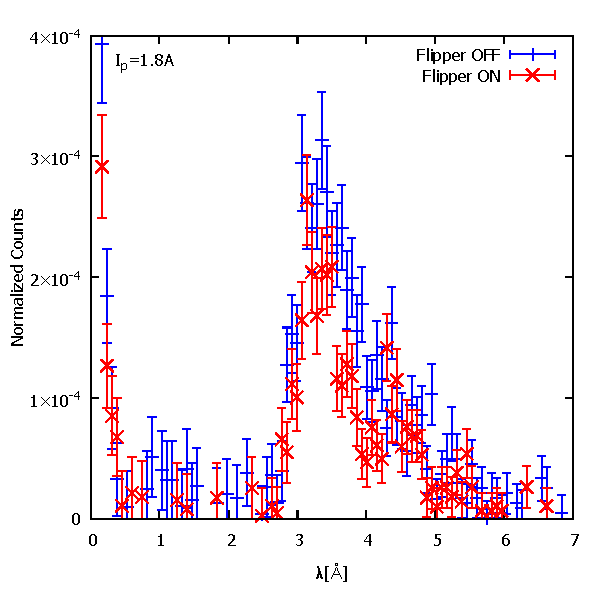
\includegraphics[width=5cm]{discussion/NC-BG/NormalizedCounts_b_18A.pdf}
\end{minipage}
\begin{minipage}{0.33\hsize}
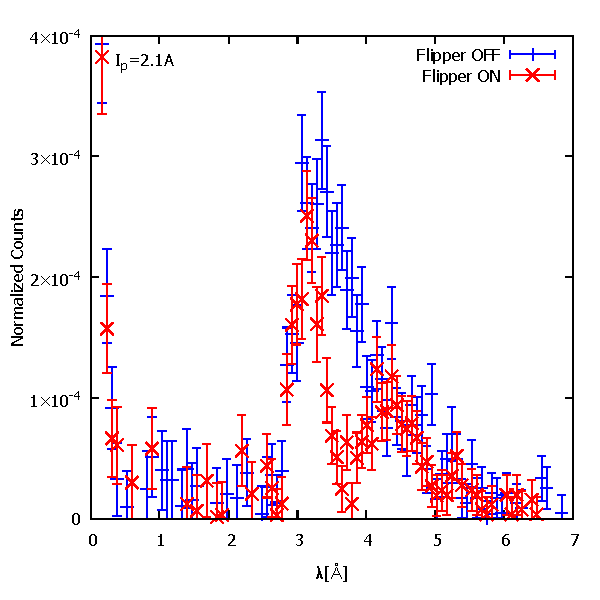
\includegraphics[width=5cm]{discussion/NC-BG/NormalizedCounts_b_21A.pdf}
\end{minipage}
\begin{minipage}{0.33\hsize}
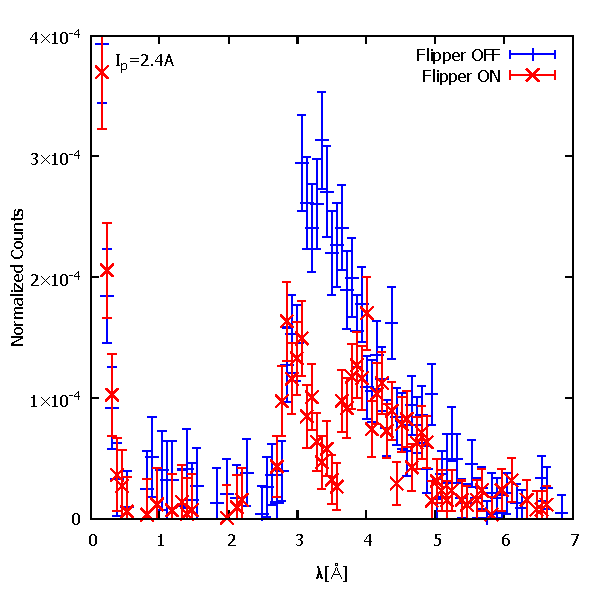
\includegraphics[width=5cm]{discussion/NC-BG/NormalizedCounts_b_24A.pdf}
\end{minipage}
\caption{規格化粒子数の波長分布(バックグラウンドを引いた後)}\label{Discussion2_fig_NC_b}
\end{figure}

\begin{figure}[h]
\begin{minipage}{0.33\hsize}
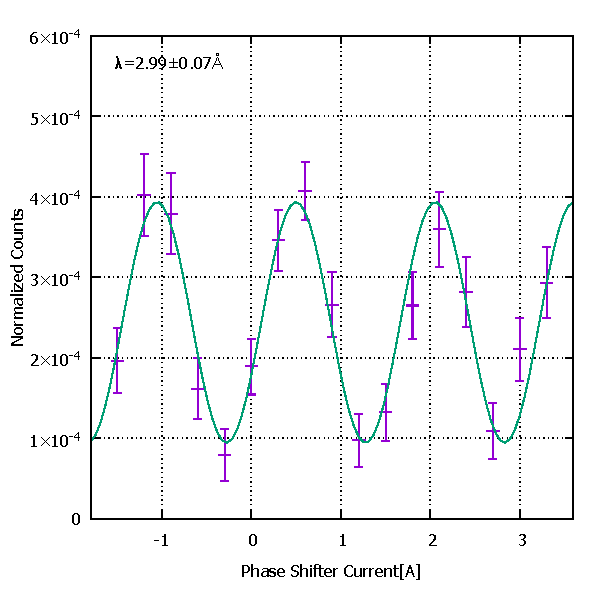
\includegraphics[width=5cm]{discussion/IF_nb/Interference_nb_fit420.pdf}
\end{minipage}
\begin{minipage}{0.33\hsize}
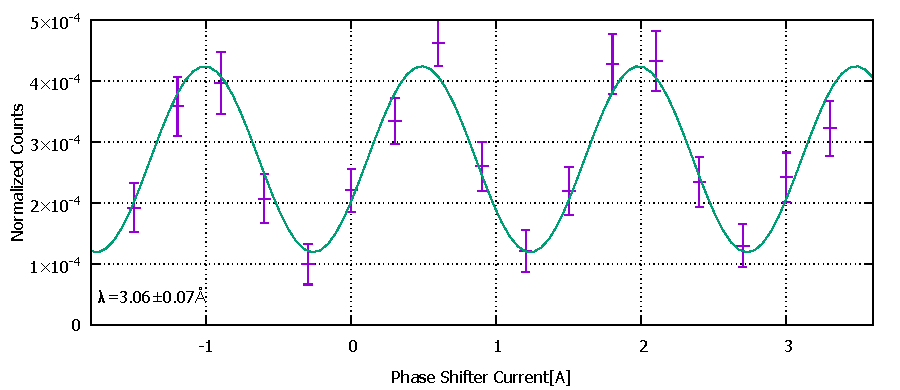
\includegraphics[width=5cm]{discussion/IF_nb/Interference_nb_fit430.pdf}
\end{minipage}
\begin{minipage}{0.33\hsize}
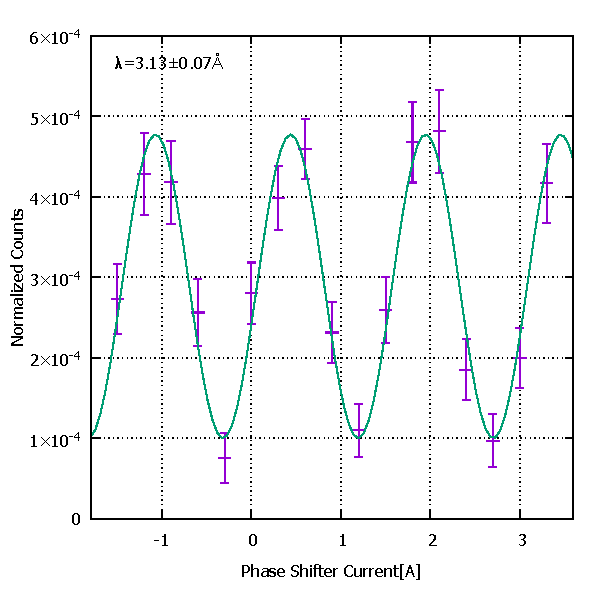
\includegraphics[width=5cm]{discussion/IF_nb/Interference_nb_fit440.pdf}
\end{minipage}\\
\begin{minipage}{0.33\hsize}
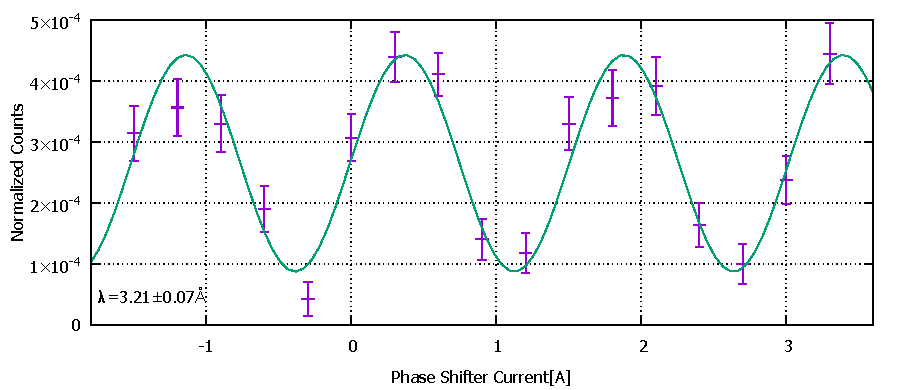
\includegraphics[width=5cm]{discussion/IF_nb/Interference_nb_fit450.pdf}
\end{minipage}
\begin{minipage}{0.33\hsize}
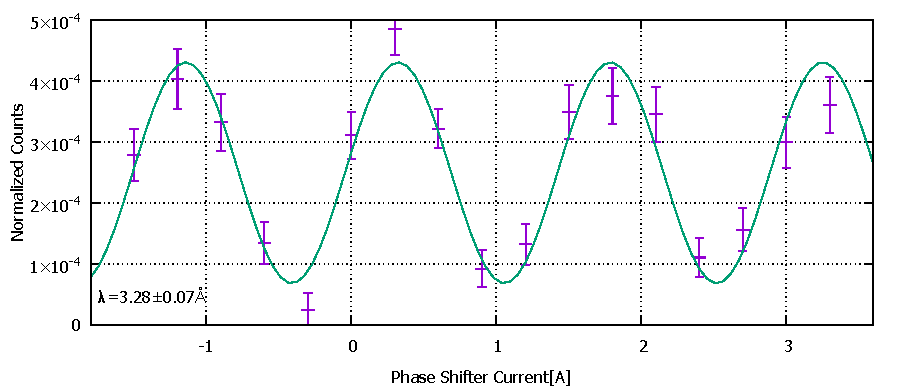
\includegraphics[width=5cm]{discussion/IF_nb/Interference_nb_fit460.pdf}
\end{minipage}
\begin{minipage}{0.33\hsize}
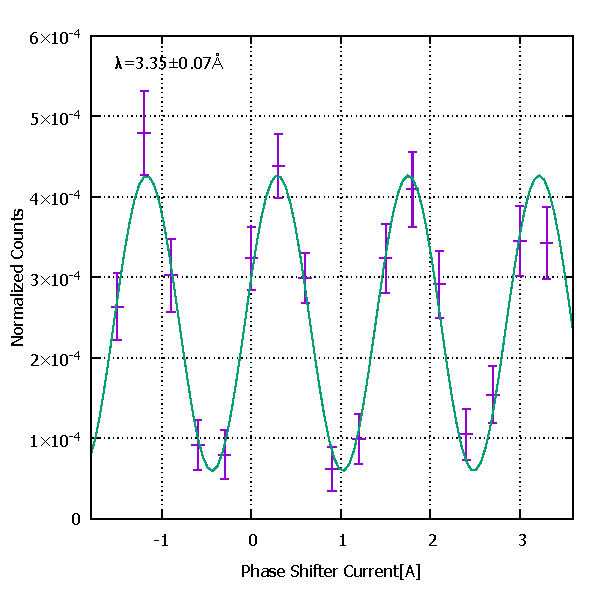
\includegraphics[width=5cm]{discussion/IF_nb/Interference_nb_fit470.pdf}
\end{minipage}\\
\begin{minipage}{0.33\hsize}
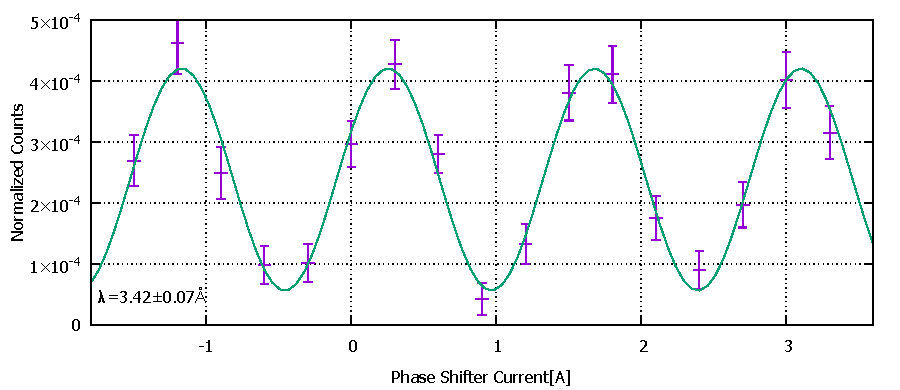
\includegraphics[width=5cm]{discussion/IF_nb/Interference_nb_fit480.pdf}
\end{minipage}
\begin{minipage}{0.33\hsize}
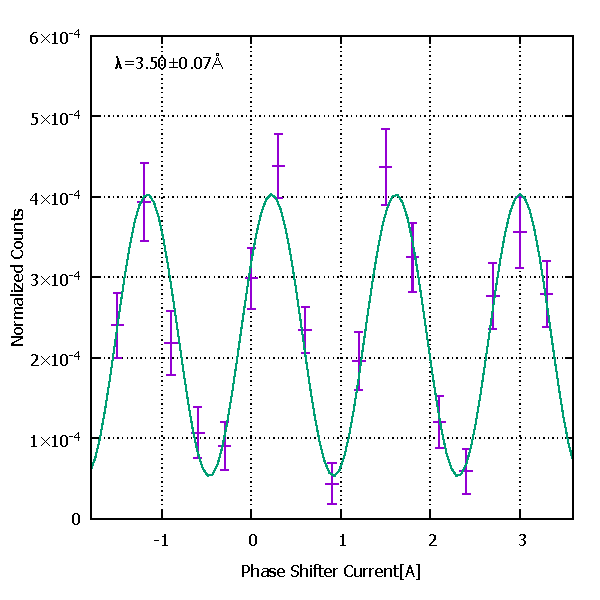
\includegraphics[width=5cm]{discussion/IF_nb/Interference_nb_fit490.pdf}
\end{minipage}
\begin{minipage}{0.33\hsize}
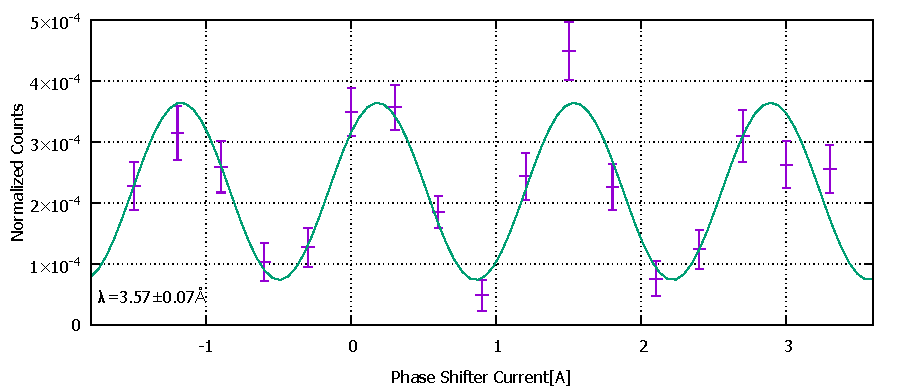
\includegraphics[width=5cm]{discussion/IF_nb/Interference_nb_fit500.pdf}
\end{minipage}\\
\begin{minipage}{0.33\hsize}
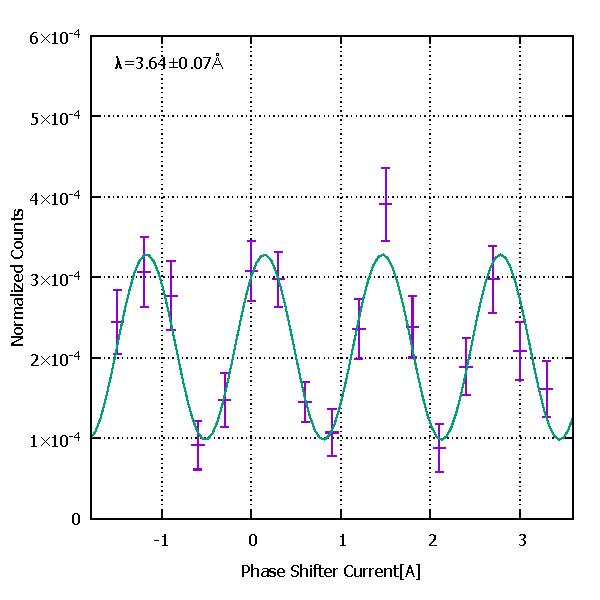
\includegraphics[width=5cm]{discussion/IF_nb/Interference_nb_fit510.pdf}
\end{minipage}
\begin{minipage}{0.33\hsize}
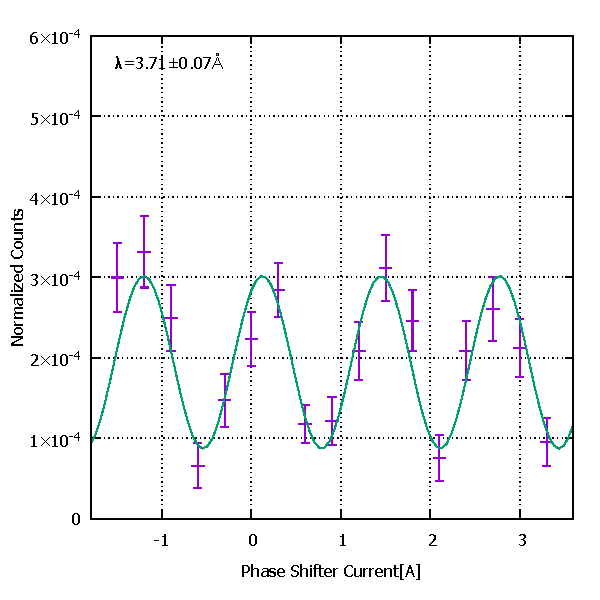
\includegraphics[width=5cm]{discussion/IF_nb/Interference_nb_fit520.pdf}
\end{minipage}
\begin{minipage}{0.33\hsize}
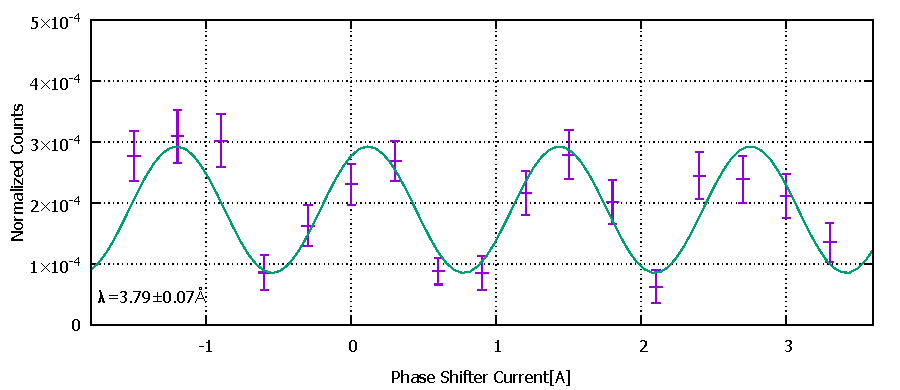
\includegraphics[width=5cm]{discussion/IF_nb/Interference_nb_fit530.pdf}
\end{minipage}
\caption{規格化粒子数の干渉パターン}\label{Discussion2_fig_IF_nb}
\end{figure}

\begin{figure}[h]
\begin{minipage}{0.33\hsize}
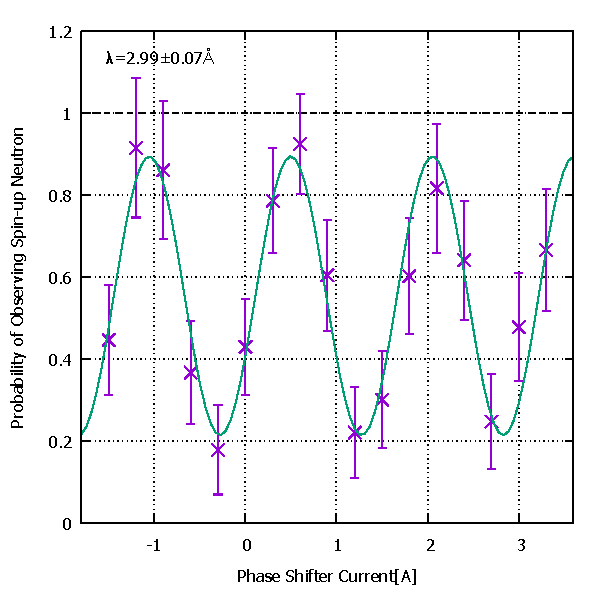
\includegraphics[width=5cm]{discussion/IF_rb/Interference_rb_fit420.pdf}
\end{minipage}
\begin{minipage}{0.33\hsize}
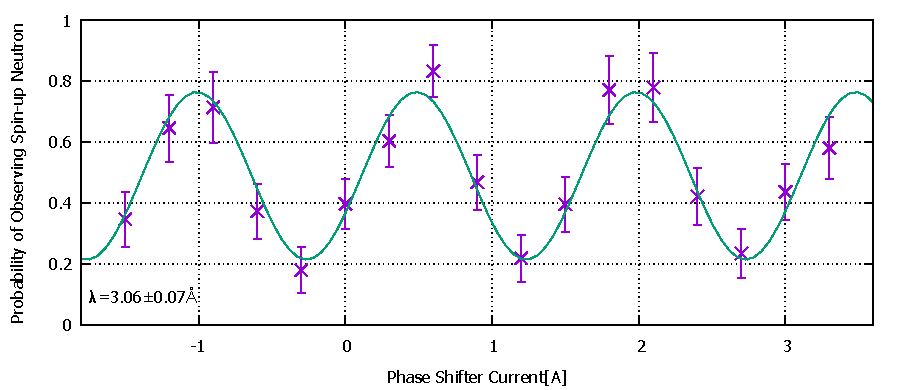
\includegraphics[width=5cm]{discussion/IF_rb/Interference_rb_fit430.pdf}
\end{minipage}
\begin{minipage}{0.33\hsize}
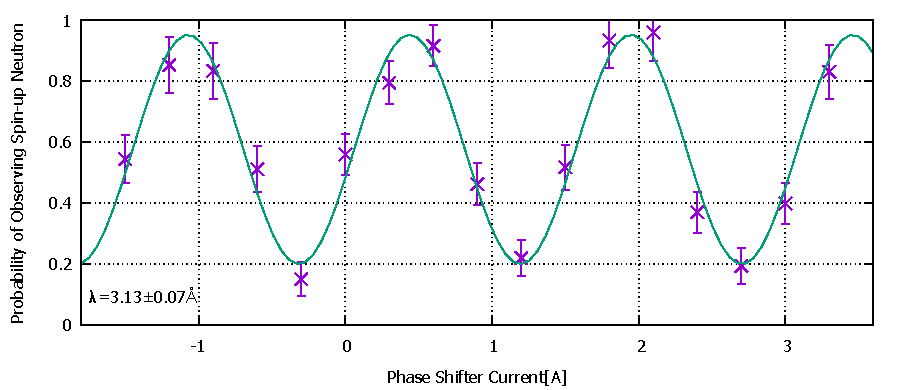
\includegraphics[width=5cm]{discussion/IF_rb/Interference_rb_fit440.pdf}
\end{minipage}\\
\begin{minipage}{0.33\hsize}
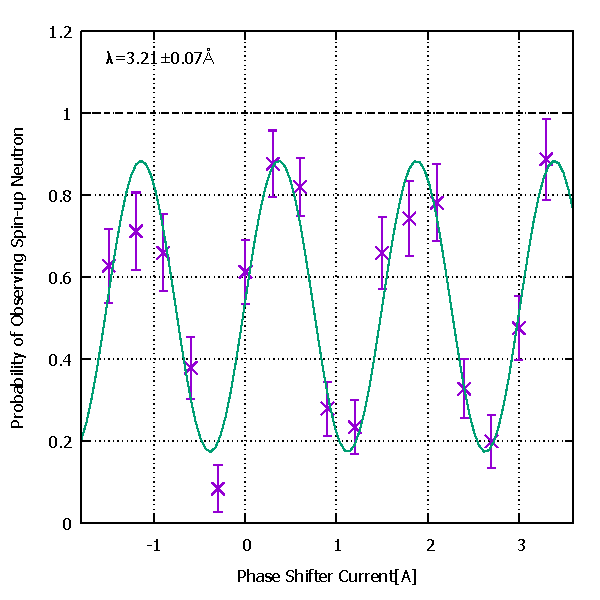
\includegraphics[width=5cm]{discussion/IF_rb/Interference_rb_fit450.pdf}
\end{minipage}
\begin{minipage}{0.33\hsize}
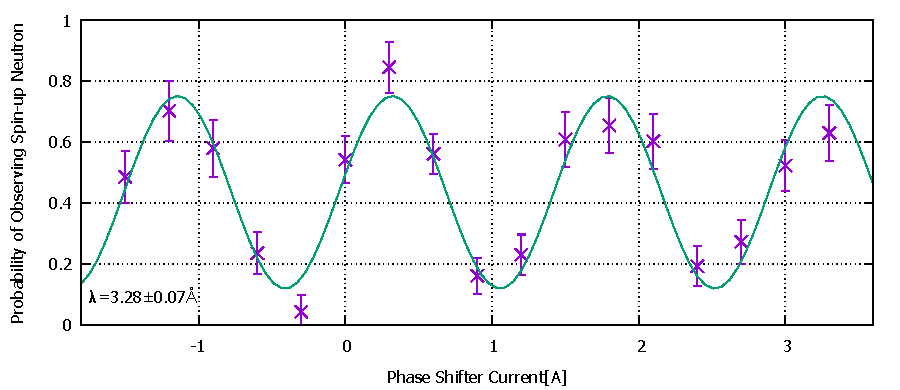
\includegraphics[width=5cm]{discussion/IF_rb/Interference_rb_fit460.pdf}
\end{minipage}
\begin{minipage}{0.33\hsize}
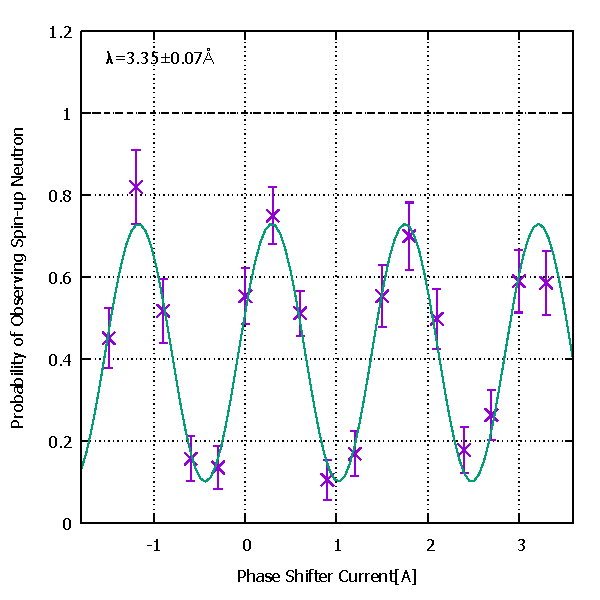
\includegraphics[width=5cm]{discussion/IF_rb/Interference_rb_fit470.pdf}
\end{minipage}\\
\begin{minipage}{0.33\hsize}
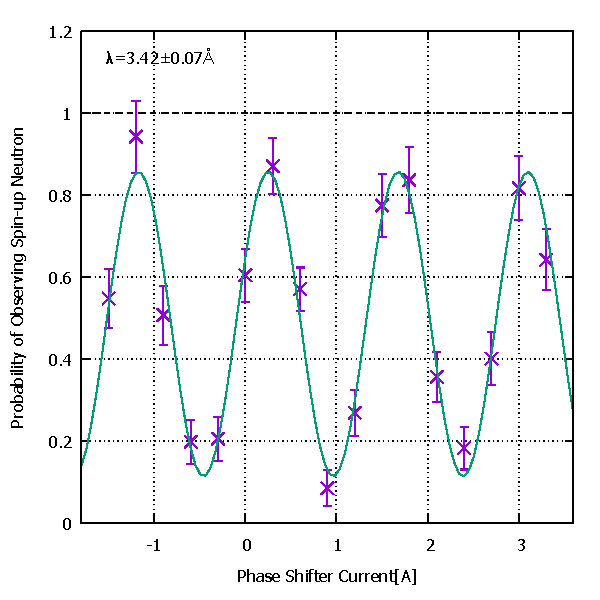
\includegraphics[width=5cm]{discussion/IF_rb/Interference_rb_fit480.pdf}
\end{minipage}
\begin{minipage}{0.33\hsize}
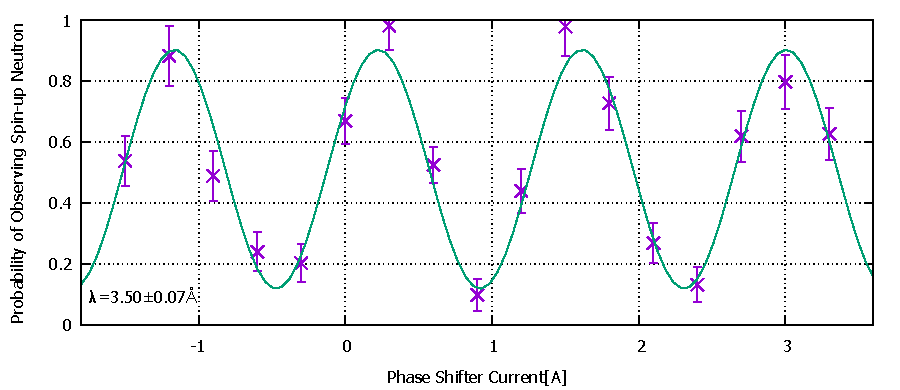
\includegraphics[width=5cm]{discussion/IF_rb/Interference_rb_fit490.pdf}
\end{minipage}
\begin{minipage}{0.33\hsize}
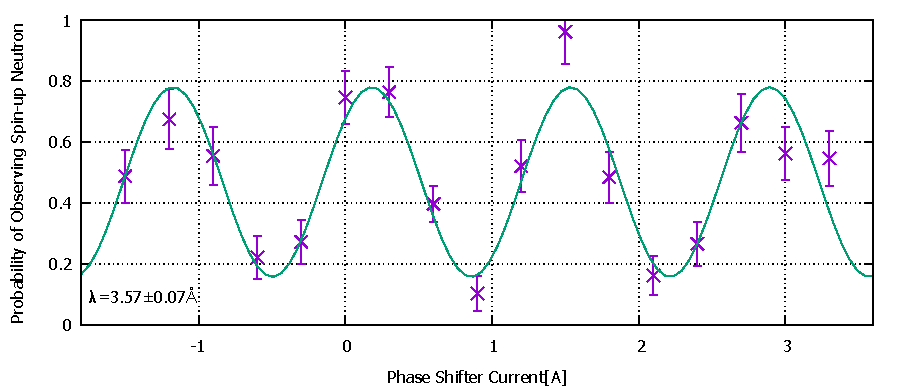
\includegraphics[width=5cm]{discussion/IF_rb/Interference_rb_fit500.pdf}
\end{minipage}\\
\begin{minipage}{0.33\hsize}
\includegraphics[width=5cm]{discussion/IF_rb/Interference_rb_fit510.pdf}
\end{minipage}
\begin{minipage}{0.33\hsize}
\includegraphics[width=5cm]{discussion/IF_rb/Interference_rb_fit520.pdf}
\end{minipage}
\begin{minipage}{0.33\hsize}
\includegraphics[width=5cm]{discussion/IF_rb/Interference_rb_fit530.pdf}
\end{minipage}
\caption{スピン上向き中性子観測確率の干渉パターン}\label{Discussion2_fig_IF_rb}
\end{figure}

\clearpage
\begin{table}[h]
\centering
\caption{各中心波長$\lambda$に対するパラメータ$A,B,C,D$とreduced$\chi^2$}
\begin{tabular}{cccccc}
$\lambda$[\AA]&$A$&$B$&$C$&$D$&reduced$\chi^2$\\ \hline
2.92 	&	0.36 	$\pm$	0.07 	&	3.84 	$\pm$	0.07 	&	0.92 	$\pm$	0.13 	&	0.76 	$\pm$	0.12 	&	0.78 	\\
2.99 	&	0.34 	$\pm$	0.05 	&	4.04 	$\pm$	0.05 	&	1.13 	$\pm$	0.09 	&	0.55 	$\pm$	0.07 	&	0.80 	\\
3.06 	&	0.27 	$\pm$	0.03 	&	4.20 	$\pm$	0.05 	&	1.11 	$\pm$	0.09 	&	0.49 	$\pm$	0.05 	&	0.75 	\\
3.13 	&	0.38 	$\pm$	0.05 	&	4.16 	$\pm$	0.04 	&	1.32 	$\pm$	0.07 	&	0.58 	$\pm$	0.06 	&	0.66 	\\
3.21 	&	0.36 	$\pm$	0.05 	&	4.16 	$\pm$	0.06 	&	1.61 	$\pm$	0.10 	&	0.53 	$\pm$	0.06 	&	1.26 	\\
3.28 	&	0.32 	$\pm$	0.04 	&	4.29 	$\pm$	0.06 	&	1.76 	$\pm$	0.10 	&	0.43 	$\pm$	0.05 	&	1.33 	\\
3.35 	&	0.31 	$\pm$	0.03 	&	4.29 	$\pm$	0.04 	&	1.89 	$\pm$	0.06 	&	0.42 	$\pm$	0.04 	&	0.58 	\\
3.42 	&	0.37 	$\pm$	0.04 	&	4.41 	$\pm$	0.04 	&	2.03 	$\pm$	0.06 	&	0.49 	$\pm$	0.05 	&	0.58 	\\
3.50 	&	0.39 	$\pm$	0.05 	&	4.52 	$\pm$	0.04 	&	2.13 	$\pm$	0.07 	&	0.51 	$\pm$	0.06 	&	0.80 	\\
3.57 	&	0.31 	$\pm$	0.05 	&	4.63 	$\pm$	0.07 	&	2.31 	$\pm$	0.11 	&	0.47 	$\pm$	0.05 	&	1.39 	\\
3.64 	&	0.27 	$\pm$	0.04 	&	4.76 	$\pm$	0.06 	&	2.45 	$\pm$	0.10 	&	0.49 	$\pm$	0.06 	&	0.70 	\\
3.71 	&	0.28 	$\pm$	0.05 	&	4.74 	$\pm$	0.09 	&	2.56 	$\pm$	0.15 	&	0.50 	$\pm$	0.06 	&	1.30 	\\
3.79 	&	0.29 	$\pm$	0.05 	&	4.76 	$\pm$	0.11 	&	2.60 	$\pm$	0.17 	&	0.53 	$\pm$	0.07 	&	1.64 	\\
3.86 	&	0.23 	$\pm$	0.04 	&	5.06 	$\pm$	0.10 	&	2.89 	$\pm$	0.16 	&	0.57 	$\pm$	0.08 	&	0.84 	\\
3.93 	&	0.29 	$\pm$	0.07 	&	5.02 	$\pm$	0.13 	&	3.44 	$\pm$	0.22 	&	0.65 	$\pm$	0.10 	&	1.72 	\\
4.00 	&	0.32 	$\pm$	0.07 	&	5.13 	$\pm$	0.08 	&	3.12 	$\pm$	0.14 	&	0.87 	$\pm$	0.15 	&	0.48 	\\ \hline
\end{tabular}
\end{table}

\paragraph{解析・考察}
バックグラウンドを考慮することによって各パラメータはどのように変わり変わらなかったのか分析を行い、その理由を考察する。
表\ref{Discussion2_tbl_ABCDb}にパラメータ$A,B,C,D$のバックグラウンド考慮前、考慮後の実験値と理論値をそれぞれ示し、その結果を図\ref{Discussion2_fig_ABCDb}に表す。表\ref{Discussion2_tbl_ABCDb}と図\ref{Discussion2_fig_ABCDb}から次のことが考察できる。
\begin{itemize}
\item パラメータ$B,C$は位相に関係した量であるからバックグラウンドによる影響はほぼなく、バックグラウンドを考慮する前と後で有効数字の範囲では誤差も含めて全く変化しない。したがって実験値と理論値はよく一致したまま保たれる。
\item パラメータ$D$は波の水深に関係する量であるからバックグラウンドの影響を受ける。バックグラウンドを考慮すると全体に小さくなる方へシフトし、3.0-3.8\AA の領域では実験値と理論値はよく一致する。領域の外では実験値が理論値よりも上へとずれてゆく。これは波長3\AA 以下や4\AA 以上では反射中性子の数が少なくなるため、下で述べるような粒子数を変化させる他の要因に強く影響されるためと考えられる。
\item パラメータ$A$も$D$と同じく波の水深に関係する量であるからバックグラウンドの影響を受ける。バックグラウンドを考慮すると、理論で予想されるまでには届かないものの、全体に上へシフトする。パラメータ$A$は位相の影響も受け、$\pm 0.07$\AA の波長領域で積分すると理論値は最大4\% 程度小さくなることを考慮すれば、理論値と実験値はさらに近づく。このようにパラメータ$A$は様々な影響を複合的に受けるためずれの原因をつきとめるのは困難であるが、次に述べるような粒子数を変化させる他の要因にも大きく影響されると考えられる。
\item 粒子数を変化させる他の要因としては、不均一磁場による軌道の変化や、空気によるスピンの反転、地磁気などの外部磁場によるスピンの反転などが考えられるが定量的な議論は難しい。
\end{itemize}

\begin{table}[H]
\caption{バックグラウンド考慮前後における実験値と理論値}\label{Discussion2_tbl_ABCDb}
\begin{minipage}{0.5\hsize}
\subcaption{$A$}
\centering
\begin{tabular}{cccc}
$\lambda$[\AA]&BG考慮前&BG考慮後&理論値\\ \hline
2.92&0.21$\pm$0.03&0.36$\pm$0.07&0.44\\
2.99 	&	0.24 	$\pm$	0.03 	&	0.34 	$\pm$	0.05 	&	0.45 	\\
3.06 	&	0.21 	$\pm$	0.02 	&	0.27 	$\pm$	0.03 	&	0.46 	\\
3.13 	&	0.28 	$\pm$	0.03 	&	0.38 	$\pm$	0.05 	&	0.47 	\\
3.21 	&	0.27 	$\pm$	0.03 	&	0.36 	$\pm$	0.05 	&	0.47 	\\
3.28 	&	0.25 	$\pm$	0.03 	&	0.32 	$\pm$	0.04 	&	0.48 	\\
3.35 	&	0.25 	$\pm$	0.02 	&	0.31 	$\pm$	0.03 	&	0.48 	\\
3.42 	&	0.29 	$\pm$	0.03 	&	0.37 	$\pm$	0.04 	&	0.49 	\\
3.50 	&	0.30 	$\pm$	0.03 	&	0.39 	$\pm$	0.05 	&	0.49 	\\
3.57 	&	0.24 	$\pm$	0.03 	&	0.31 	$\pm$	0.05 	&	0.49 	\\
3.64 	&	0.21 	$\pm$	0.03 	&	0.27 	$\pm$	0.04 	&	0.50 	\\
3.71 	&	0.21 	$\pm$	0.03 	&	0.28 	$\pm$	0.05 	&	0.50 	\\
3.79 	&	0.22 	$\pm$	0.04 	&	0.29 	$\pm$	0.05 	&	0.50 	\\
3.86 	&	0.17 	$\pm$	0.03 	&	0.23 	$\pm$	0.04 	&	0.50 	\\
3.93 	&	0.21 	$\pm$	0.04 	&	0.29 	$\pm$	0.07 	&	0.50 	\\
4.00 	&	0.21 	$\pm$	0.03 	&	0.32 	$\pm$	0.07 	&	0.50	\\ \hline
\end{tabular}
\vspace{5mm}
\end{minipage}
\begin{minipage}{0.5\hsize}
\subcaption{$B$}
\centering
\begin{tabular}{cccc}
$\lambda$[\AA]&BG考慮前&BG考慮後&理論値\\ \hline
2.92&3.84$\pm$0.07&3.84$\pm$0.07&3.71\\
2.99 	&	4.04 	$\pm$	0.05 	&	4.04 	$\pm$	0.05 	&	3.81 	\\
3.06 	&	4.20 	$\pm$	0.05 	&	4.20 	$\pm$	0.05 	&	3.90 	\\
3.13 	&	4.16 	$\pm$	0.04 	&	4.16 	$\pm$	0.04 	&	3.99 	\\
3.21 	&	4.16 	$\pm$	0.06 	&	4.16 	$\pm$	0.06 	&	4.08 	\\
3.28 	&	4.29 	$\pm$	0.06 	&	4.29 	$\pm$	0.06 	&	4.18 	\\
3.35 	&	4.29 	$\pm$	0.04 	&	4.29 	$\pm$	0.04 	&	4.27 	\\
3.42 	&	4.41 	$\pm$	0.04 	&	4.41 	$\pm$	0.04 	&	4.36 	\\
3.50 	&	4.52 	$\pm$	0.04 	&	4.52 	$\pm$	0.04 	&	4.45 	\\
3.57 	&	4.63 	$\pm$	0.07 	&	4.63 	$\pm$	0.07 	&	4.54 	\\
3.64 	&	4.76 	$\pm$	0.06 	&	4.76 	$\pm$	0.06 	&	4.64 	\\
3.71 	&	4.74 	$\pm$	0.09 	&	4.74 	$\pm$	0.09 	&	4.73 	\\
3.79 	&	4.76 	$\pm$	0.11 	&	4.76 	$\pm$	0.11 	&	4.82 	\\
3.86 	&	5.06 	$\pm$	0.10 	&	5.06 	$\pm$	0.10 	&	4.91 	\\
3.93 	&	5.02 	$\pm$	0.13 	&	5.02 	$\pm$	0.13 	&	5.01 	\\
4.00 	&	5.13 	$\pm$	0.08 	&	5.13 	$\pm$	0.08 	&	5.10 	\\ \hline
\end{tabular}
\vspace{5mm}
\end{minipage}\\
\begin{minipage}{0.5\hsize}
\subcaption{$C$}
\centering
\begin{tabular}{cccc}
$\lambda$[\AA]&BG考慮前&BG考慮後&理論値\\ \hline
2.92&0.92$\pm$0.13&0.92$\pm$0.13&0.71\\
2.99 	&	1.13 	$\pm$	0.09 	&	1.13 	$\pm$	0.09 	&	0.89 	\\
3.06 	&	1.11 	$\pm$	0.09 	&	1.11 	$\pm$	0.09 	&	1.07 	\\
3.13 	&	1.32 	$\pm$	0.07 	&	1.32 	$\pm$	0.07 	&	1.25 	\\
3.21 	&	1.61 	$\pm$	0.10 	&	1.61 	$\pm$	0.10 	&	1.43 	\\
3.28 	&	1.76 	$\pm$	0.10 	&	1.76 	$\pm$	0.10 	&	1.61 	\\
3.35 	&	1.89 	$\pm$	0.06 	&	1.89 	$\pm$	0.06 	&	1.80 	\\
3.42 	&	2.03 	$\pm$	0.06 	&	2.03 	$\pm$	0.06 	&	1.98 	\\
3.50 	&	2.13 	$\pm$	0.07 	&	2.13 	$\pm$	0.07 	&	2.17 	\\
3.57 	&	2.31 	$\pm$	0.11 	&	2.31 	$\pm$	0.11 	&	2.35 	\\
3.64 	&	2.45 	$\pm$	0.10 	&	2.45 	$\pm$	0.10 	&	2.54 	\\
3.71 	&	2.56 	$\pm$	0.15 	&	2.56 	$\pm$	0.15 	&	2.72 	\\
3.79 	&	2.60 	$\pm$	0.17 	&	2.60 	$\pm$	0.17 	&	2.91 	\\
3.86 	&	2.89 	$\pm$	0.16 	&	2.89 	$\pm$	0.16 	&	3.10 	\\
3.93 	&	3.44 	$\pm$	0.22 	&	3.44 	$\pm$	0.22 	&	3.29 	\\
4.00 	&	3.12 	$\pm$	0.14 	&	3.12 	$\pm$	0.14 	&	3.48 	\\ \hline
\end{tabular}
\end{minipage}
\begin{minipage}{0.5\hsize}
\subcaption{$D$}
\centering
\begin{tabular}{cccc}
$\lambda$[\AA]&BG考慮前&BG考慮後&理論値\\ \hline
2.92&0.85$\pm$0.08&0.76$\pm$0.12&0.55\\
2.99 	&	0.69 	$\pm$	0.06 	&	0.55 	$\pm$	0.07 	&	0.54 	\\
3.06 	&	0.61 	$\pm$	0.05 	&	0.49 	$\pm$	0.05 	&	0.54 	\\
3.13 	&	0.68 	$\pm$	0.05 	&	0.58 	$\pm$	0.06 	&	0.53 	\\
3.21 	&	0.64 	$\pm$	0.05 	&	0.53 	$\pm$	0.06 	&	0.52 	\\
3.28 	&	0.55 	$\pm$	0.04 	&	0.43 	$\pm$	0.05 	&	0.52 	\\
3.35 	&	0.53 	$\pm$	0.04 	&	0.42 	$\pm$	0.04 	&	0.51 	\\
3.42 	&	0.60 	$\pm$	0.05 	&	0.49 	$\pm$	0.05 	&	0.51 	\\
3.50 	&	0.62 	$\pm$	0.05 	&	0.51 	$\pm$	0.06 	&	0.50 	\\
3.57 	&	0.58 	$\pm$	0.05 	&	0.47 	$\pm$	0.05 	&	0.50 	\\
3.64 	&	0.61 	$\pm$	0.05 	&	0.49 	$\pm$	0.06 	&	0.50 	\\
3.71 	&	0.62 	$\pm$	0.06 	&	0.50 	$\pm$	0.06 	&	0.50 	\\
3.79 	&	0.65 	$\pm$	0.06 	&	0.53 	$\pm$	0.07 	&	0.50 	\\
3.86 	&	0.68 	$\pm$	0.07 	&	0.57 	$\pm$	0.08 	&	0.50 	\\
3.93 	&	0.75 	$\pm$	0.08 	&	0.65 	$\pm$	0.10 	&	0.50 	\\
4.00 	&	0.92 	$\pm$	0.10 	&	0.87 	$\pm$	0.15 	&	0.50 	\\ \hline
\end{tabular}
\end{minipage}
\end{table}

\begin{figure}[H]
\begin{center}
\includegraphics[width=12cm]{discussion/ABCD/A_ab.pdf}
\subcaption{$A$}
\vspace{1cm}
\includegraphics[width=12cm]{discussion/ABCD/B_ab.pdf}
\subcaption{$B$}
\end{center}
%\end{minipage}\\
%\begin{minipage}{0.5\hsize}
\caption{バックグラウンド考慮前後における実験値の比較}\label{Discussion2_fig_ABCDb}
\end{figure}
\begin{figure}[H]
\begin{center}
\ContinuedFloat
\includegraphics[width=12cm]{discussion/ABCD/C_ab_fit.pdf}
\subcaption{$C$}
\vspace{1cm}
\includegraphics[width=12cm]{discussion/ABCD/D_ab.pdf}
\subcaption{$D$}
\end{center}
\caption{バックグラウンド考慮前後における実験値の比較}\label{Discussion2_fig_ABCDb}
%\end{minipage}
\end{figure}

\subsection{波の合成}
\ref{Analysis_sec}章のはじめに、実験で得た干渉の波を4つのパラメータに分解した。それ以降干渉波を波としては扱わず、意味のはっきりした要素毎に取り扱った。そうすることで複合的な問題が分割されてシンプルなものとなり、容易に解析を進めることができた。しかし小さなことばかりに集中していると視野が狭くなり、全体像が見えづらくなる。ここでは分解した波を再び合成することで、広い視野で全体を見通してゆく。

\paragraph{全体像}
これまでの解析の流れを波の観点から眺めてみる。

\begin{figure}[h]
\begin{minipage}{0.49\hsize}
\centering
\includegraphics[width=\hsize]{discussion/SEA/IT_0_480.pdf}
\caption{シンプルな場合}\label{Discussion2_fig_wave_simple}
\includegraphics[width=\hsize]{discussion/SEA/IT_e_480.pdf}
\caption{共鳴からのずれを考慮}\label{Discussion2_fig_waveve_resonance}
\includegraphics[width=\hsize]{discussion/SEA/IT_eb_480.pdf}
\caption{バックグラウンドを考慮}\label{Discussion2_fig_wave_background}
\end{minipage}
\hspace{2mm}
\begin{minipage}{0.49\hsize}
\begin{enumerate}
\item 実験で得られた干渉波のデータは、共鳴条件を満たすとしたと最もシンプルな理論では説明が付かない。波の振動数に関しては実験値と理論値で近いように思われるが、位相のずれのせいではっきりしない(図\ref{Discussion2_fig_wave_simple})。
\item そこで共鳴条件からのずれを考えることにより、波の位相をあわせることができる。しかし同時に振幅や振動中心も動くため解析は難しい。これで振動数と位相ずれは理論から説明することができる(図\ref{Discussion2_fig_waveve_resonance})。
\item 振幅と振動中心のずれが気になるが、波そのものを見ているとバックグラウンドの存在に気づきやすい。バックグラウンドを考慮することで実験値の波としてのふるまいを理論である程度説明することができる(図\ref{Discussion2_fig_wave_background})。
\end{enumerate}
このように波そのものを扱うと次にどうすべきかの見通しは非常によい。しかし定量的な議論は困難であり、またパラメータのときのように同時に複数の波長に対して解析することは難しい。

このような理由から波を分解して解析する手法をとった。しかし全体像の把握は常に必要である。
\vspace{4.5cm}
\end{minipage}
\end{figure}

\paragraph{広い視野}
これまでは分解した要素と理論値を対応させるために狭い波長領域しか考えることができなかった。しかし波を波として捉えればどんな波長領域でも扱うことができる。中心波長$\lambda=3.42$\AA に対して領域$\pm 0.07,\pm0.14,\pm0.22,\pm0.29,\pm0.36,\pm0.43,\pm0.51$\AA を取ったときの実験値と理論値は次の図\ref{Discussion2_fig_around480}のようになる。波長領域を広げることで位相のずれが大きくなり、うなりのように振幅が変動する様子が実験値からはっきりと見て取れる。また理論がそれを精度よく予測していることも注目に値する。
\begin{figure}[H]
\centering
%\begin{minipage}{0.5\hsize}
\includegraphics[width=9cm]{discussion/SEA/IT_480_10.pdf}
%\end{minipage}
%\begin{minipage}{0.5\hsize}
\includegraphics[width=9cm]{discussion/SEA/IT_480_20.pdf}
%\end{minipage}\\
%\begin{minipage}{0.5\hsize}
\includegraphics[width=9cm]{discussion/SEA/IT_480_30.pdf}
%\end{minipage}
%\begin{minipage}{0.5\hsize}
\includegraphics[width=9.cm]{discussion/SEA/IT_480_40.pdf}
\caption{広い波長領域における実験値と理論値}
\end{figure}
\begin{figure}[H]
\ContinuedFloat
\centering
%\end{minipage}\\
%\begin{minipage}{0.5\hsize}
\includegraphics[width=9cm]{discussion/SEA/IT_480_50.pdf}
%\end{minipage}
%\begin{minipage}{0.5\hsize}
\includegraphics[width=9cm]{discussion/SEA/IT_480_60.pdf}
%\end{minipage}\\
%\begin{minipage}{0.5\hsize}
\includegraphics[width=9cm]{discussion/SEA/IT_480_70.pdf}
%\end{minipage}
\caption{広い波長領域における実験値と理論値}
\end{figure}

\subsection{まとめ}
実験でせっかく得られた干渉の波は\ref{Analysis_sec}章のはじめに4つに分解された。それは波模様という漠然とした概念を実体があり形の分かる要素に分けることで、ゆれる波に惑わされることなく地に足を付けて解析を進めるためであった。しかし足下ばかり見ていては全体像が見えづらくなる。ここでは分解した波を再び合成し、広い視野を持って干渉の海原を見渡してゆく。








